\begin{center}
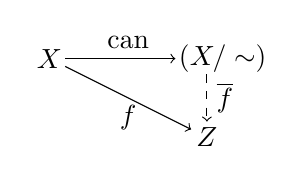
\begin{tikzpicture}
  \filldraw (0,0)node{$X$} circle (0pt);
  \filldraw (2.2,0)node{$(X/\sim)$} circle (0pt);
  \filldraw (2,-1)node{$Z$} circle (0pt);
  \draw[->] (0.2, 0) -- (1.6,0);
  \draw[->] (0.2,-0.1) -- (1.8,-0.9);
  \draw[->,dashed] (2,-0.2) -- (2,-0.8);
  \filldraw (1,0)node[anchor=south]{can} circle (0pt);
  \filldraw (2,-.5)node[anchor=west]{$\overline{f}$} circle (0pt);
  \filldraw (1,-.75)node{$f$} circle (0pt);
\end{tikzpicture}
\end{center}